\documentclass[spec, och, labwork]{shiza}
% параметр - тип обучения - одно из значений:
%    spec     - специальность
%    bachelor - бакалавриат (по умолчанию)
%    master   - магистратура
% параметр - форма обучения - одно из значений:
%    och   - очное (по умолчанию)
%    zaoch - заочное
% параметр - тип работы - одно из значений:
%    referat    - реферат
%    coursework - курсовая работа (по умолчанию)
%    diploma    - дипломная работа
%    pract      - отчет по практике
% параметр - включение шрифта
%    times    - включение шрифта Times New Roman (если установлен)
%               по умолчанию выключен
\usepackage{subfigure}
\usepackage{tikz,pgfplots}
\pgfplotsset{compat=1.5}
\usepackage{float}

%\usepackage{titlesec}
\setcounter{secnumdepth}{4}
%\titleformat{\paragraph}
%{\normalfont\normalsize}{\theparagraph}{1em}{}
%\titlespacing*{\paragraph}
%{35.5pt}{3.25ex plus 1ex minus .2ex}{1.5ex plus .2ex}

\titleformat{\paragraph}[block]
{\hspace{1.25cm}\normalfont}
{\theparagraph}{1ex}{}
\titlespacing{\paragraph}
{0cm}{2ex plus 1ex minus .2ex}{.4ex plus.2ex}

% --------------------------------------------------------------------------%


\usepackage[T2A]{fontenc}
\usepackage[utf8]{inputenc}
\usepackage{graphicx}
\graphicspath{ {./images/} }
\usepackage{tempora}

\usepackage[sort,compress]{cite}
\usepackage{amsmath}
\usepackage{amssymb}
\usepackage{amsthm}
\usepackage{fancyvrb}
\usepackage{listings}
\usepackage{listingsutf8}
\usepackage{longtable}
\usepackage{array}
\usepackage[english,russian]{babel}

% \usepackage[colorlinks=true]{hyperref}
\usepackage{url}

\usepackage{underscore}
\usepackage{setspace}
\usepackage{indentfirst} 
\usepackage{mathtools}
\usepackage{amsfonts}
\usepackage{enumitem}
\usepackage{tikz}
\usepackage{minted}

\newcommand{\eqdef}{\stackrel {\rm def}{=}}
\newcommand{\specialcell}[2][c]{%
\begin{tabular}[#1]{@{}c@{}}#2\end{tabular}}

\renewcommand\theFancyVerbLine{\small\arabic{FancyVerbLine}}

\newtheorem{lem}{Лемма}

\begin{document}

% Кафедра (в родительном падеже)
\chair{}

% Тема работы
\title{Логические элементы и схемы}

% Курс
\course{3}

% Группа
\group{331}

% Факультет (в родительном падеже) (по умолчанию "факультета КНиИТ")
\department{факультета КНиИТ}

% Специальность/направление код - наименование
%\napravlenie{09.03.04 "--- Программная инженерия}
%\napravlenie{010500 "--- Математическое обеспечение и администрирование информационных систем}
%\napravlenie{230100 "--- Информатика и вычислительная техника}
%\napravlenie{231000 "--- Программная инженерия}
\napravlenie{10.05.01 "--- Компьютерная безопасность}

% Для студентки. Для работы студента следующая команда не нужна.
% \studenttitle{Студентки}

% Фамилия, имя, отчество в родительном падеже
\author{Стаина Романа Игоревича и Токарева Никиты Сергеевича}

% Заведующий кафедрой
% \chtitle{} % степень, звание
% \chname{}

%Научный руководитель (для реферата преподаватель проверяющий работу)
\satitle{аспирант} %должность, степень, звание
\saname{А. А. Мартышкин}

% Руководитель практики от организации (только для практики,
% для остальных типов работ не используется)
% \patitle{к.ф.-м.н.}
% \paname{С.~В.~Миронов}

% Семестр (только для практики, для остальных
% типов работ не используется)
%\term{8}

% Наименование практики (только для практики, для остальных
% типов работ не используется)
%\practtype{преддипломная}

% Продолжительность практики (количество недель) (только для практики,
% для остальных типов работ не используется)
%\duration{4}

% Даты начала и окончания практики (только для практики, для остальных
% типов работ не используется)
%\practStart{30.04.2019}
%\practFinish{27.05.2019}

% Год выполнения отчета
\date{2022}

\maketitle

% Включение нумерации рисунков, формул и таблиц по разделам
% (по умолчанию - нумерация сквозная)
% (допускается оба вида нумерации)
% \secNumbering

%-------------------------------------------------------------------------------------------
\section{Цель работы:}

Ознакомление с основными характеристиками логических элементов и основами синтеза логических схем.

\textbf{Задание 1.}

Построим схему основных и базовых логических элементов.

    \begin{figure}[H]
        \centering      %размер рисунка       здесь находится название файла рисунка, без указания формата
        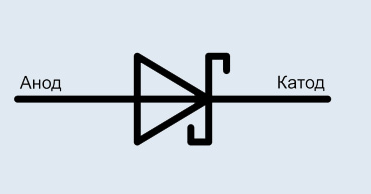
\includegraphics[width=0.7\textwidth]{1}
        \caption{Реализация схемы из задания 1}
        \label{fig:image1}
    \end{figure}
        
    Оперируя ключами 1, 2, …, 9 сформируем все возможные комбинации аргументов х1 и х2 (00, 01, 10, 11) на входе 
    дизъюнктора (OR), конъюнктора (AND), штриха Шеффера (NAND) и стрелки Пирса (NOR) и запишем значения выходных 
    логических функций ук (0 или 1) в таблицу.

    \begin{figure}[H]
        \centering      %размер рисунка       здесь находится название файла рисунка, без указания формата
        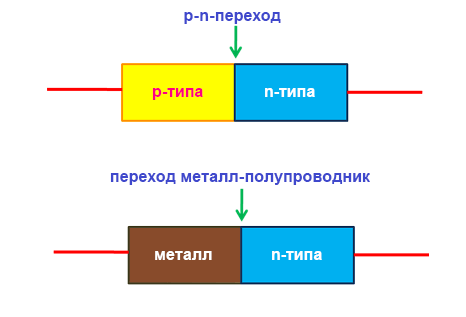
\includegraphics[width=0.7\textwidth]{2}
        \caption{Таблица всех возможных комбинаций аргументов}
        \label{fig:image1}
    \end{figure}
        
\textbf{Задание 2.}

Соберем схему для реализации заданной логической функции y = (ab + ¬c)( ¬a + ¬b + c)(a + b + c)

    \begin{figure}[H]
        \centering      %размер рисунка       здесь находится название файла рисунка, без указания формата
        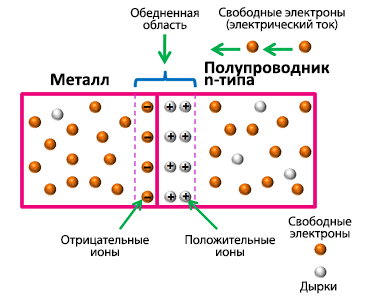
\includegraphics[width=1.\textwidth]{3}
        \caption{Реализация схемы из задания 2}
        \label{fig:image1}
    \end{figure}

Функция равна нулю при любых входных сигналах.

\textbf{Вывод:} ознакомились с основными характеристиками логических элементов и основами синтеза логических схем.\\

\section{Тестовые задания к работе 29:}

\begin{enumerate}
    \item Укажите признаки характеризующие основные логические элементы:
    
    Ответ:
    \begin{itemize}
        \item используя основные логические операции И, ИЛИ и НЕ, можно аналитически
        выразить любую сложную логическую функцию;
        \item минимальный логический базис составляют операции ИЛИ и НЕ или И и НЕ;
        \item входные и выходные сигналы логических элементов могут принимать только
        два значения: логическую 1 и логический 0.
    \end{itemize}

    \item Укажите выражение логической функции двух переменных х1 и х2, реализуемой элементом «стрелка Пирса»:
    
    Ответ: $y = \overline{x_1 + x_2}$.

    \item Укажите выражение логической функции двух переменных х1 и х2, реализуемой элементом «штрих Шеффера»:
    
    Ответ: $y = \overline{x_1x_2}$.

    \item Укажите выражение логической функции трех переменных а, б и с, записанной
    в совершенной дизъюнктивной нормальной форме (СДНФ):

    Ответ: $y(a, b, c) = \overline{a}bc + a\overline{b}c + ab\overline{c} + abc$.

    \item Укажите элемент ИЛИ-НЕ:
    
    Ответ: на рисунке 4 представлен элемент ИЛИ-НЕ.

    \begin{figure}[H]
        \centering      %размер рисунка       здесь находится название файла рисунка, без указания формата
        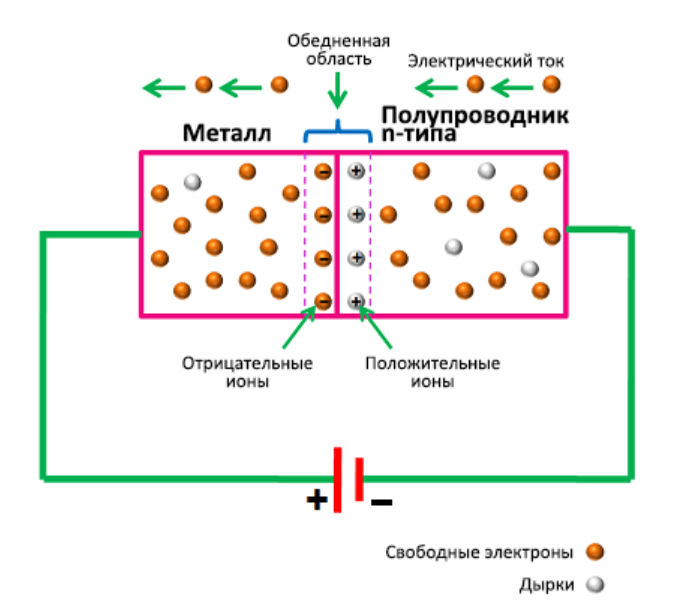
\includegraphics[width=0.4\textwidth]{4}
        \caption{Элемент ИЛИ-НЕ}
        \label{fig:image1}
    \end{figure}

    \item Укажите элемент И:
    
    Ответ: на рисунке 5 показан элемент И.

    \begin{figure}[H]
        \centering      %размер рисунка       здесь находится название файла рисунка, без указания формата
        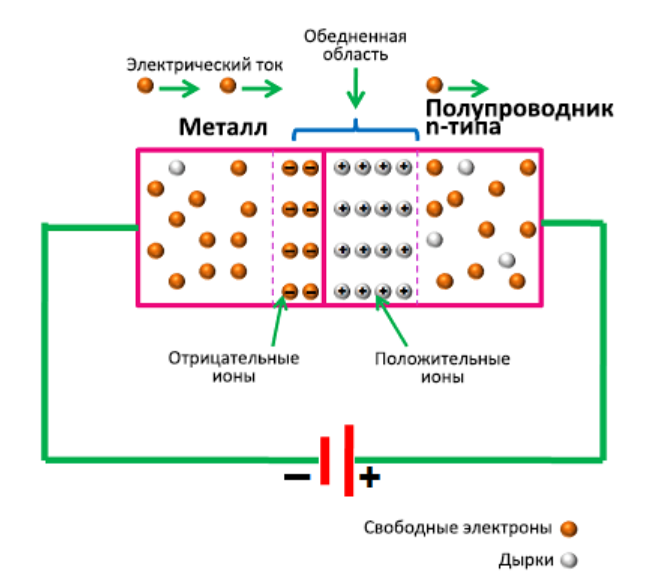
\includegraphics[width=0.4\textwidth]{5}
        \caption{Элемент И}
        \label{fig:image1}
    \end{figure}

    \item Укажите значение функции $y = (ab + \overline{c})(\overline{a} + \overline{b})$ если а = b = с = 1:
    
    Ответ: 0.
\end{enumerate}

\end{document}
